%
% File acl2010.tex
%
% Contact  jshin@csie.ncnu.edu.tw or pkoehn@inf.ed.ac.uk
%%
%% Based on the style files for ACL-IJCNLP-2009, which were, in turn,
%% based on the style files for EACL-2009 and IJCNLP-2008...

%% Based on the style files for EACL 2006 by 
%%e.agirre@ehu.es or Sergi.Balari@uab.es
%% and that of ACL 08 by Joakim Nivre and Noah Smith

\documentclass[a4paper,11pt]{article}
\usepackage{acl2010}
\usepackage{times}
\usepackage{float}
\usepackage{url}
\usepackage{latexsym}
\usepackage{epsfig}
\usepackage{latexsym}
\usepackage[usenames]{color}
\usepackage{times} 
\usepackage{verbatim}
\usepackage{multirow}
\usepackage{threeparttable}
\usepackage{booktabs}
%\setlength\titlebox{6.5cm}    % You can expand the title box if you
% really have to

\title{The C-Cat Wordnet Package: An Open Source Package for modifying and
applying Wordnet}

\author{ Keith Stevens and Terry Huang\\
  Department of Computer Science\\
  University of California, Los Angeles, 90095\\
  {\tt \{kstevens,thuang513\}@cs.ucla.edu} \And
  David Buttler \\
  Center for Applied Scientific Computing\\
  LLNL, Livermore 94550\\
  {\tt buttler1@llnl.gov} 
  }

\date{}

\begin{document}
\maketitle
\begin{abstract}

We present the C-Cat Wordnet package, an open source library for using and
modifying Wordnet.  The package includes four key features: an API for modifying Synsets; implementations of standard similarity
metrics, implementations of well-known Word Sense Disambiguation algorithms, and an
implementation of the Castanet algorithm.  The library is easily extendible and usable in many runtime environments.  We demonstrate it's use on two standard Word Sense Disambiguation tasks and apply the Castanet algorithm to a corpus.
\end{abstract}

\section{Introduction}

Wordnet \cite{fellbaum98wordnet} is a hierarchical lexical database that provides a fine grained semantic interpretation of a word. 
Wordnet forms a diverse semantic network by first collecting similar words into synonym sets ($Synset$), for example ``drink'' and ``imbibe'' are connected under the verb $Synset$ defined as ``take in liquids.''  Then, $Synsets$ are connected by relational links, with the IS-A link being the most well known.

% Summarize the current libraries.
Applications typically access Wordnet through one or more libraries.  Every popular programming language has at least one library: the original for C++, JWNL \footnote{http://sourceforge.net/projects/jwordnet/} for Java, and
WordNet::QueryData \footnote{http://people.csail.mit.edu/jrennie/WordNet/} for
Perl are just a few examples.  While these libraries are robust and provide many features, they cannot be easily applied to two new use cases: direct modification and serialization of the database and use in a parallel processing framework, such the Hadoop \footnote{http://hadoop.apache.org/} framework.  The first has become a popular research topic in recent years, with \newcite{snow06extwn} providing a well known method for adding new lexical mappings to Wordnet, and the second will increasingly become important as Wordnet applications are applied to massive web-scale datasets.

% Highlight why we wrote the package.  What are it's main goals.
We developed the C-Cat Wordnet package to address these use cases as part
of a larger information extraction and retrieval system that requires word sense information for new, domain specific terms and novel composite senses on web-scale corpora.  One example includes adding new lexical mappings harvested from New York Times articles.  Without support for saving additions to Wordnet and parallel processing, we would be unable to leverage existing valuable sense information.  Our package solves these issues with a new API focused on modifying the database and by storing the
entire Wordnet database in memory.

%, which separates lexical queries from file systems and makes possible dynamic modification of the hierarchy.  

We designed the package to be a flexible library for any Wordnet application.  It is written in Java and defines a standard Java interface for core data structures and algorithms.  All code has been heavily documented with details on performance trade-offs and unit tested to ensure reliable behavior.  While other Wordnet libraries exist, we hope that the release of ours facilitates the development of new, customized Wordnets and the use of Wordnet in large highly parallelized systems.   The toolkit is available at {\small \url{http://github.com/fozziethebeat/C-Cat}}, which include a wiki detailing the
structure of the package, javadocs, and a mailing list.

\section{The C-Cat Wordnet Framework}

Fundamentally, Wordnet acts as a mapping from word forms to possible word senses.  Terms with similar senses are collapsed into a single $Synset$.  The $Synset$ network is then formed by linking a $Synset$ to others via semantic links such as IS-A, PART-OF, and SIMILAR-TO. Our package makes two significant contributions: a collection a standardized reference implementations of well known algorithms and a new API for directly modifying and serializing the $Synset$ network.  Furthermore, it stores the hierarchy in memory, separating lexical queries from disc access and allows for serialization of modified hierarchies.  Lastly, it provides features found in comparable libraries such as JWNL.

%Our API introduces new methods for modifying this semantic structure.  Any modification can be saved to the standard Wordnet data format, which can later be %read by our library or any other Wordnet library.

The C-Cat library is split up into four packages:
\begin{enumerate}
{\small
\item The Core API contains data format readers, writers, and $Synsets$;
\item Similarity Metrics;
\item Word Sense Disambiguation algorithms;
\item and Castanet \cite{stoica07automatingcreation}, a method for automatically learning document
facets using Wordnet.
}
\end{enumerate}

\subsection{Core API}

The core API is centered around two interfaces: an $OntologyReader$ and a
$Synset$.  The $OntologyReader$ is responsible for parsing a Wordnet file
format, building a linked $Synset$ network, and returning $Synsets$ based on
query terms and parts of speech.  The $Synset$ maintains all of the information
for a particular word sense, such as it's definitions, examples, and links to
other $Synsets$. Both interfaces provide mechanisms for modifying the sense
information, $Synset$ links, and lexical mappings.  We store this entire
structure in memory due to the minimal size of Wordnet, for example, version 3.0
is only 37 Megabytes on disk, and so that users can use Wordnet on novel
distributed file systems, such as Hadoop, that do not use standard file system
APIs.

\paragraph{$Synsets$} are defined by three sets of values: word forms, links to other $Synsets$, and a part of speech.  Each $Synset$ may have
multiple word forms and multiple links, but only one part of speech.  
We use both standard Wordnet relations and arbitrary relations to label a directed link between two $Synsets$, with the relation being stored in only the source $Synset$.  
We provide several methods for accessing relations and related $Synsets$: $getKnownRelationTypes()$, $allRelations()$, and $getRelations()$. 
In addition, each $Synset$ can have
a set of example sentences and a definition.  To modify each $Synset$,
the interface includes additive methods for relations, word forms, and examples.  Furthermore,
we provide a $merge()$ method that takes all information from one $Synset$ and adds it to another $Synset$.   Figure \ref{fig:merge}
provides a simple example using this merge API; after the code has been run, ``cat.n.1'' will contain all of the information from it's related $Synsets$.
Lastly, the interface also permits arbitrary objects, such as ranking values,
feature vectors, or additional meta data, to be attached
to any $Synset$ as an $Attribute$.  Any $Attributes$ are also merged on a call to $merge$. 

\begin{figure}
\small
\begin{verbatim}
OntologyReader reader = ...
Synset cat = reader.getSynset("cat.n.1");
for (Synset rel : cat.allRelations())
  cat.merge(rel);
System.out.println(cat);
\end{verbatim}
\caption{A simple merge example using the $OntologyReader$ and $Synset$ interfaces.}
\label{fig:merge}
\end{figure}

\paragraph{$OntologyReader$} defines an interface that maps word forms to $Synset$s.  Implementations are designed to be initialized once and then used ubiquitously throughout an application.  The interface provides methods for getting all $Synset$s for a word or a specific sense, for
example, the query ``cat.n.1'' in figure \ref{fig:merge} retrieves the first noun $Synset$ for the term ``cat''.  
To modify the sense network, we provide two key methods: $addSynset(new)$ and $removeSynset(old)$.  $addSynset(new)$ adds a mapping from each of $new$'s word forms to $new$. $removeSynset(old)$ removes all mappings from $old$'s word forms to $old$, thus removing it from the lexical mapping completely.

\subsection{Similarity Metrics}

\begin{figure*}
\small
\begin{verbatim}
OntologyReader reader = WordNetCorpusReader.initialize(...);
Set<Sysnet> nouns = reader.allSynsets(PartsOfSpeech.NOUN);
SynsetSimilarity sims[] = {new PathSimilarity(), new LeskSimilarity(), ...};
for (Synset s1 : nouns)
  for (Synset s2 : nouns)
    for (SynsetSimilarity sim : sims)
      System.out.printf("%s %s %f\n", s1, s2, sim.similarity(s1, s2));
\end{verbatim}
\caption{Code for computing the pairwise similarity over every noun $Synset$ using multiple metrics}
\label{fig:sim}
\end{figure*}

While the semantic network of Wordnet is interesting on it's own, many
applications require sense similarity measures.  As such, we provide the
$SynsetSimilarity$ interface that
returns a similarity score between two $Sysnet$s.  This is, in short, a Java
based implementation of the Wordnet::Similarity package \cite{pedersen04sim}, which is in
Perl.  Figure \ref{fig:sim} provides a naive, but short, code sample of our API that computes the similarity between all noun $Synset$s using multiple metrics.

Below, we briefly summarize the measures from \cite{pedersen04sim} that we implemented. Several measures utilize the Lowest Common Subsumer (LCS), i.e. the deepest parent common to two $Synset$s using IS-A relations. Each measure takes in two $Synset$s, $A$ and $B$, as arguments and returns a double value, typically between 0 and 1.

\paragraph{Path Based Methods} measure the similarity based on a path connecting $A$ and $B$.  $Path$ simply returns the inverse length of the shortest path between $A$ and $B$.  $Leacock \& Chodorow$ \cite{Leacock98sim} returns the length of the shortest path scaled by the deepest depth in the hierarchy.  $Wu \& Palmer$ \cite{wu94sim} returns the depth of the LCS scaled by the cumulative depth of $A$ and $B$.  $Hirst \& St. Onge$ \cite{hirst97lexical} uses all links in the hierarchy and measures the length of the path that is both short and has very few link types.

\paragraph{Lexical methods} measure the amount of lexical overlap between $A$ and $B$.  $Lesk$ \cite{lesk86wsd} returns the number of words overlapping in $A$ and $B$'s glosses.  $ExtendedLesk$ \cite{banerjee03extlesk} extends Lesk by also comparing the glosses between any $Synset$s related to $A$ or $B$.

\paragraph{Information based Methods} utilize the Information Content (IC) of a $Synset$, which measures the specificity of the terms in a $Synset$ as measured in a sense tagged corpus.  $Resnick$ \cite{Resnik95sim} returns the IC of the LCS.  $Jiang \& Conrath$ \cite{jiang97taxonomySimilarity} returns the inverse difference between the total IC of $A$ and $B$ and the IC of their LCS.  $Lin$ \cite{Lin98sim} returns the IC of the LCS scaled by the total IC of $A$ and $B$.

In addition to the raw similarity metrics, we provide a utility classes that return
meta information about a pair of $Sysnets$ such as their shortest path, their
LCS, and several other helpful methods.

\subsection{Word Sense Disambiguation}

Word Sense Disambiguation is perhaps the most standard application of Wordnet.  Disambiguation models attempt to select a $Synset$ for a given word that best matches a given context.  For example, an algorithm might select the river bank $Synset$ of  ``bank'' for the context ``he sat on the bank of the river'' rather than the financial institution $Synset$.  We provide a $WordSenseDisambiguation$ interface that applies word sense labels to tokenized sentences.  Currently, we only provide a small number of unsupervised algorithms, but plan on adding more.  Below, we briefly describe each algorithm.

\paragraph{Lexical Methods} rely on lexical information in Wordnet to disambiguate words.  $Lesk$ \cite{lesk86wsd} selects the $Synset$ that has the highest total Lesk similarity to the $Synset$s for other context words.  $ExtendedLesk$ \cite{banerjee03extlesk} extends Lesk by using the Extended Lesk similarity metric for all comparisons.  $MostFrequentSense$ selects the first $Synset$ returned by Wordnet for a given term.  This serves as a canonical baseline which is often challenging to outperform.

\paragraph{Graphical Methods} treat the network as a graph and disambiguate using a number of measurements.  $PersonalizedPageRank$ \cite{agirre09wsd} ($PPR$) runs the PageRank algorithm over an undirected graph composed from the entire Wordnet network.  Words needing disambiguation are given ``artificial'' nodes that link to their possible $Synset$s.  For each ambiguous word, the algorithm selects the highest ranking $Synset$.  $DegreeCentrality$ \cite{navigli10graph} ($DC$) forms a subgraph from the Wordnet network composed of ambiguous content words in a sentence and the $Synset$s that connect their possible $Synset$s.  It assigns to each word the target $Synset$ with the highest degree in the subgraph. $PageRankCentrality$ \cite{navigli10graph} ($PRC$) composes the same subgraph as $DegreeCentrality$, but performs PageRank on this subgraph and selects the $Synset$ with the highest rank for each ambiguous word.

\subsection{Castanet}

Amazon.com and other online retailers often display manually crafted facets, or
categories, for product navigation.  A customer can start browsing from the Book
category and dive down into more specific categories such as Fiction,
Entertainment, or Politics.  These facets form a hierarchy of categories and
each category is subdivided until a narrow set of interesting items are found.
Unfortunately, not all datasets have well structured meta data.  The Castanet
algorithm automatically learns this hierarchical faceted meta data (HFC) for a
set of documents by using discriminative keywords
\cite{stoica07automatingcreation}, making structured navigation possible for
arbitrary document sets.

Castanet takes advantage of Wordnet’s IS-A hierarchy to automatically create HFC. Castanet first extracts keywords from the set of documents (we use term-frequency inverse document frequency, TF-IDF, by default, but our API allows for other methods). For each extracted keyword, Castanet then creates a chain of words that lead from the root of the hierarchy to the keyword's $Synsets$. Each keyword chain is then merged together to form a ``backbone'' tree which is later reduced by eliminating redundant or non-discriminative nodes, such as those with one child.

Our Castanet API is both simple and flexible. To create a Castanet tree, one calls $Castanet.buildTree()$ with a directory path to a set of text documents.  Our implementation will automatically extract keywords, extract the backbone tree, and finally index each document under it's learned facets.  The returned result allows users to fully navigate the documents via the learned facets.  We also provide an example Java web service for exploring the hierarchy in a browser.

\section{Benchmark}

To evaluate our library, we apply our six WSD implementations against two standard evaluations: the all words disambiguation tasks from SenseEval 3 \cite{snyder-palmer:2004:Senseval-3} and SemEval 2007 \cite{pradhan07semeval}, these use Wordnet version 1.7.1 and 2.1 respectively.  We answer all test instances except those that do not have any mapping in Wordnet.  Before processing, we apply part of speech tags to each token using the Open NLP MaxEnt Tagger ver 1.5.0\footnote{http://opennlp.sourceforge.net/models-1.5/}.   We use the original databases as a baseline, called Base, in our experiments and test our modification API by adding the eXtended Wordnet (XWN) relations \cite{mihalcea01extendedwordnet} to each database and disambiguate using these extended Wordnets\footnote{Note that we added XWN 1.7 relations to Wordnet 1.7.1 and XWN 2.0 relations to Wordnet 2.1, some links were discarded due to updates in Wordnet.}.

\begin{table}[h]
\small
\center
\begin{tabular}{|c|c|c|c|}
\hline
Model & Ver & SenseEval-3 & SemEval-07 \\
\hline
MFS & Base & 59.8 & 49.4 \\
\hline
Lesk & Base & 35.2 & 27.7 \\
E-Lesk & Base & 47.8 & \bf{37.6} \\
PPR & Base & 42.9 & 32.8  \\
DC & Base & 43.2 & 33.3 \\
PRC & Base & 31.7 & 22.7 \\
\hline
Lesk & XWN & 35.2 & 27.7 \\
E-Lesk & XWN & 39.9 & 33.9 \\
PPR & XWN & \bf{50.3} & 36.7  \\
DC & XWN & 47.3 & 37.1 \\
PRC & XWN & 33.0 & 24.0 \\
\hline
\end{tabular}
\caption{F1 Word Sense Disambiguation scores on the two test sets}
\label{tab:wsd}
\end{table}

Table \ref{tab:wsd} presents the F1 score for each algorithm using the original and extended databases.  As expected, the MFS baseline outperforms each unsupervised algorithm.  Although our scores do not match exactly with previous publications of these algorithms, we still see similar trends and the expected gains from adding new relations to the hierarchy.  For $DegreeCentrality$ and $PageRankCentrality$, our different results are likely due to a implementation difference: when extracting a subgraph from Wordnet, we only use directed links as opposed to undirected links for computational efficiency.  Other variations are possibly due to different methods of handling multi-word expressions and our part of speech tags.  Still, $DC$ gains about 4\% points with WXN relations and $PPR$ gains about 7\% points on Senseval-3.  Unexpectedly, $ExtendedLesk$ actually does worse with the additional relations.  

We also performed a visual test of our Castanet implementation.  We ran the algorithm over 1,021 articles extracted from the BBC World News using Wordnet 3.0. The articles came from a diverse set of categories including world, business, technology, and environmental news. Figures \ref{fig:casta1} and \ref{fig:casta2} show snapshots of our Castanet web application. Figure \ref{fig:casta1} displays the top level facets displayed to a new user.  The top bar of this screen can break down the facets alphabetically to facilitate facet selection.  Figure \ref{fig:casta2} shows a snapshot of several documents found after selecting several facets.  It displays the selected facets, document titles, document text, and interesting key words.                  While this is only a simple interface, it provides an example of what our implementation can accomplish and how to use our API.

\section{Future Work and Conclusion}

We have presented our Java Wordnet library that provides two new key features: maintenance of an in memory database and an API centered around modifying the network directly.  Additionally, we've provided implementations of several well known similarity metrics, disambiguation algorithms, and the Castanet information retrieval algorithm.  All code is unit tested, heavily documented, and released under the GPL Version 2 license.  We are currently working to extend our newest APIs, such as those for WSD and Castanet, to handle more interesting use cases.  In the future work we hope to expand this library with an evaluation framework for customized Wordnets, such as those generated by \cite{snow06extwn}.

\begin{figure*}[h!]
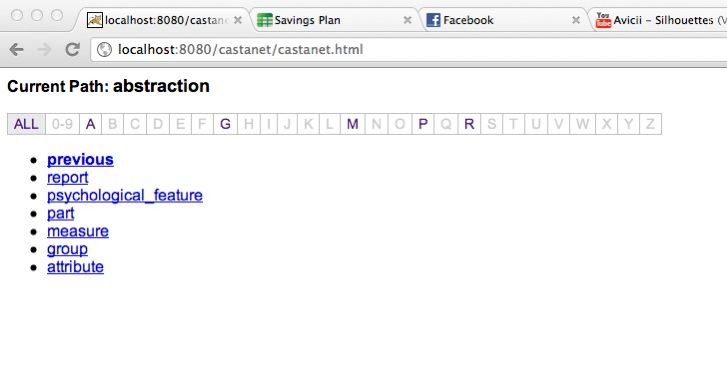
\includegraphics[width=1.0\textwidth]{new_castanet3.jpg}
\caption{A sample view of learned Castanet facets for the BBC Word News data set}
\label{fig:casta1}
\end{figure*}

\begin{figure*}[h!]
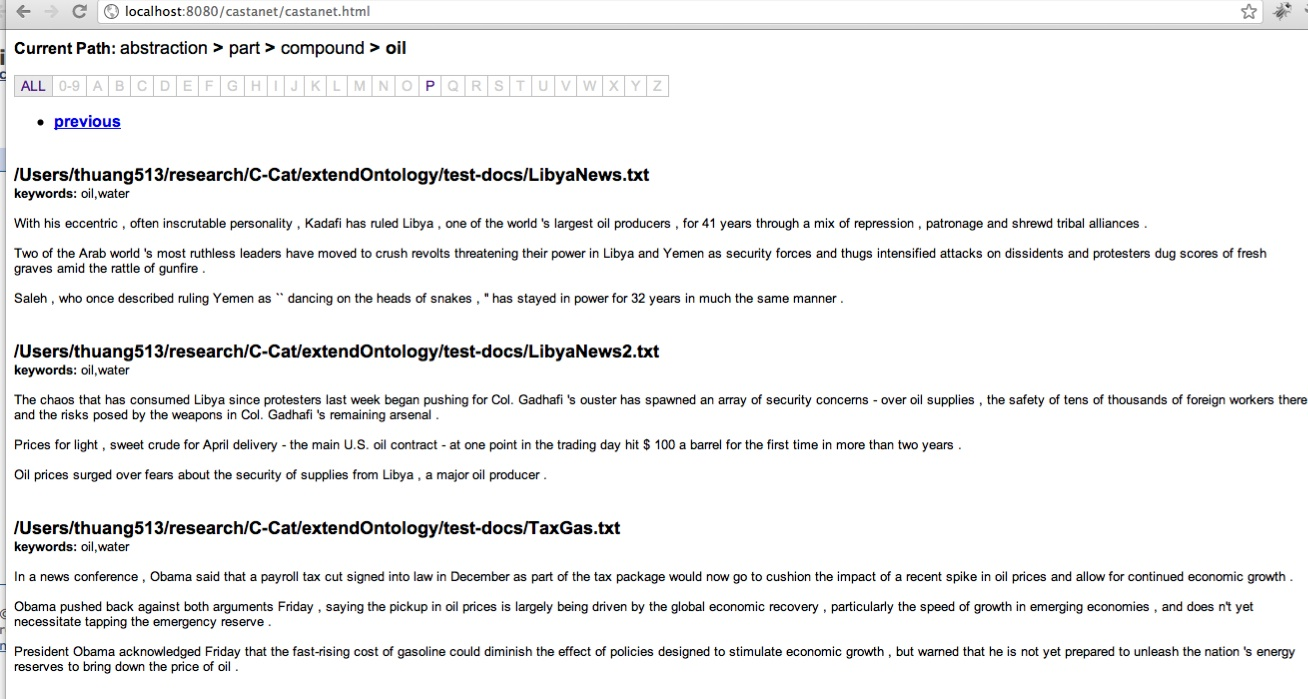
\includegraphics[width=1.0\textwidth]{new_castanet4.jpg}
\caption{A sample view of a discovered document after navigating the Castanet facets}
\label{fig:casta2}
\end{figure*}

\paragraph{Acknowledgements} This work was performed under the auspices of the U.S. Department of Energy by Lawrence Livermore National Laboratory under Contract DE-AC52-07NA27344 (LLNL-CONF-499791).

\bibliographystyle{acl}
\bibliography{gwa12}

\end{document}
